%%%%%%%%%%%%%%%%%%%%% chapter1.tex %%%%%%%%%%%%%%%%%%%%%%%%%%%%%%%%%
%
%  
%
% Use this file as a template for your own input.
%
%%%%%%%%%%%%%%%%%%%%%%%% Springer-Verlag %%%%%%%%%%%%%%%%%%%%%%%%%%
%\motto{Use the template \emph{chapter.tex} to style the various elements of your chapter content.}






\section{Summary of Module}
\label{sec:1}

 We are interested in approaches to the fundamental hardness questions in computational complexity.

Computational complexity: the study of which problems can be efficiently computed and which cannot.

Efficiency: we understand efficiency as Polynomial Time computability. A Boolean function $f:\{0,1\}^n\to\{0,1\}$ is said to be efficiently computable if there is a polynomial-time Turing Machine M that, on input $x$ in $\bits^n$ outputs $f(x)$ and runs in time $n^c$ for some constant $c$. Note that $n^c$ is a polynomial in the input length $n$ (the exponent $c$ does not depend on the input length $n$). 

The arguably main question of the theory of computation, the one that subsumes in some sense many problems in other parts of computing, once is the \P~vs~\NP~question: Can we separate \P~from \NP, namely, is there a language in \NP~ that is not in \P? In other words, can we prove that SAT (Boolean satisfiability problem) cannot be solved in polynomial time? And yet again, roughly, can problems whose solutions once given can be verified efficiently, can be solved efficiently? 

We are interested in \emph{concrete} approaches, namely, considering a simple, usually combinatorial-looking, model of computation, such as a Boolean circuit, and establishing lower bounds against the size of circuits required to prove certain specific functions that are given to us concretely (usually, these functions also possess some straightforward combinatorial 
properties; e.g., they represented specific graph problems). In this sense, the question is concrete because the result is unconditional (namely, it does not depend on unproved 
assumptions, such as $\P\neq\NP$), and the model itself is concrete: it is a (primarily combinatorial) object of which its size we lower 
bound in precise terms (e.g., circuit $C$ computing function $f(x)$ must have size $2^{|x|}$, where $|x|$ is the bit-size of the input $x$).
\medskip 

Three main concrete approaches to the fundamental hardness questions are the following:

\begin{enumerate}
\item  Circuit Complexity 
\item Proof Complexity 
\item Algebraic Complexity
\end{enumerate}

We shall see a bit from each, mainly circuit complexity and some basic proof complexity while commenting briefly on algebraic complexity. 



Other approaches to the fundamental hardness questions are usually more intrinsic to complexity theory. In that respect, the whole of computational complexity theory could be viewed as ``approaching" the fundamental hardness questions through complexity class, reductions, concrete lower bounds and the relation between these notions and results. One intriguing approach that makes this attempt in particular is the ``Meta Complexity" approach. We are not going to touch on this in this course. 



\chapter{Introduction to Circuit Complexity}
\label{intro} % Always give a unique label
% use \chaptermark{}
% to alter or adjust the chapter heading in the running head
 

\section{Basic Circuit Complexity}
\label{sec:2}
% Always give a unique label
% and use \ref{<label>} for cross-references
% and \cite{<label>} for bibliographic references
% use \sectionmark{}
% to alter or adjust the section heading in the running head

\begin{definition}[Boolean Circuit]
Let $n \in \mathbb{N}$ and $x_1, \ldots, x_n$ be $n$ variables. A Boolean Circuit $C$ with $n$ inputs is a directed acyclic graph. It contains $n$ nodes with no incoming edges, called the \emph{input nodes} and a single node with no outgoing edges, called the \emph{output node}.
All other nodes are \emph{internal nodes} or \emph{gates}, and
are labelled by the logical gates $\lor, \land,\neg$ (i.e., logical OR, AND, NOT, resp.). The $\lor,\land$ nodes have fan-in (i.e., number of incoming nodes) 2, and $\neg$ has fan-in 1. The \emph{size of $C$}, denoted $|C|$, is the number of nodes in the underlying graph.
$C$ is called a \emph{formula} if each node has at most one outgoing edge (i.e., the underlying graph is a tree),
\end{definition}




\begin{figure}
\sidecaption
  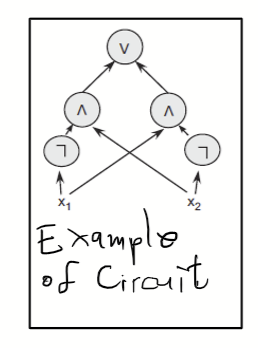
\includegraphics[width=0.2\linewidth]{images/Example-circuit.png}
    \caption{Example of a simple Boolean circuit.}
    \label{fig:enter-label}
\end{figure}

%

\subparagraph{Comment}
Fan-in $d>2$ 
can be simulated by a tree of $d-1 $ nodes: 
\begin{figure}[h]
    \centering
  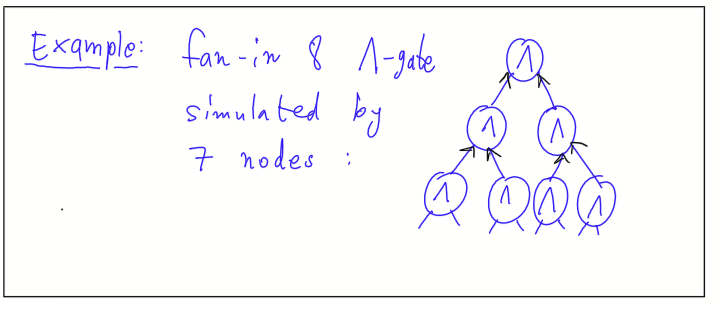
\includegraphics[width=0.5\linewidth]{images/Example-tree-circuit.png}
    \label{fig:enter-label}
\end{figure}
 


\newpage 
 

% Define a question counter
\newcounter{questcounter}
\renewcommand{\thequestcounter}{\arabic{questcounter}} 
 
% Define the numbered question environment
\newenvironment{myquestion}{%
    \refstepcounter{questcounter} % Increment counter for referencing
    \begin{svgraybox}
    \noindent\textbf{Question~\thequestcounter:} % Code at the beginning
    \end{svgraybox}}{%
    \par % Code at the end (e.g., end with a paragraph break)
}
 
 
\begin{myquestion}{What is the function computed by the circuit below?}
\label{quest:1}
\begin{figure}
    \centering
    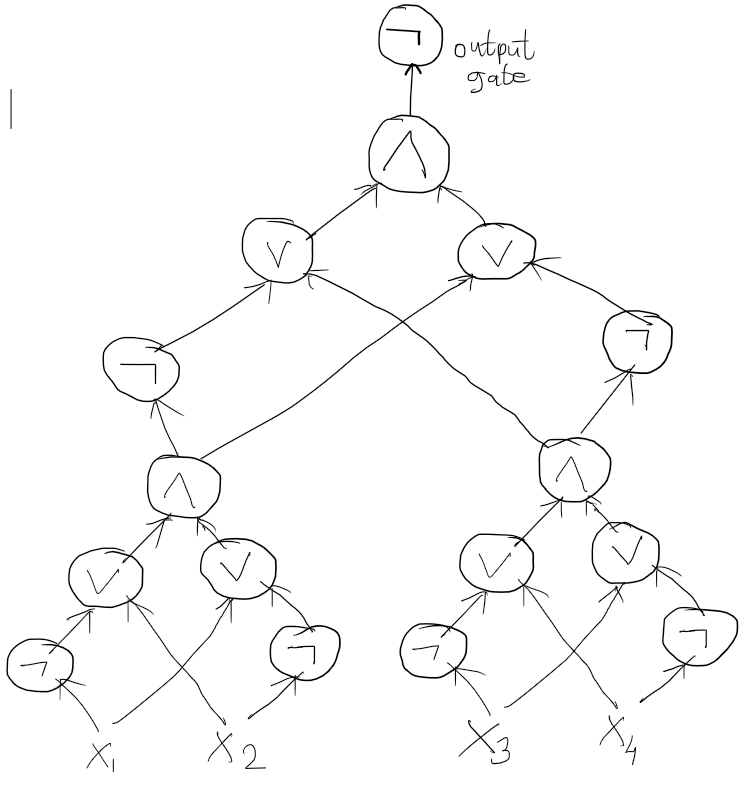
\includegraphics[width=0.75\linewidth]{images/parity-circuit-question.png}
    \caption{Question}
    \label{fig:enter-label}
\end{figure}
\end{myquestion}
 
See the answer at the  end of the chapter (page \pageref{trailer:xor-circuit}).



\section{Basic concepts: circuit families, language recognition, and function computation}

Let $\mathbb{N}$ denote the set of natural numbers starting from $1$.


%\newcommand{\bits}{\ensuremath{\{0,1\}}}
%\newcommand{\demph}[1]{\textbf{\emph{#1}}}

A \emph{language} is a set of (finite) strings. Note that the language can contain infinite many strings, only that each string is finite. A \emph{string} is an ordered sequence of symbols from a fixed constant size alphabet. We shall use mainly strings over the alphabet consisting of two symbols $\bits$.
Hence, a language is simply a set $L\subseteq\bits^*$ (recall, that $\bits^*$ is the set of all finite 0-1 strings, including the empty string). 
 

\begin{tcolorbox}[float=t, colframe=white, colback=red!5, boxrule=0mm, sharp corners]
\begin{definition}
Let $T:\mathbb{N}\rightarrow \mathbb{N}$ be a function. 
A \emph{$T(n)$-\textbf{sized circuit family}} is a sequence $\left\{C_n\right\}_{n \in \mathbb{N}}$ of Boolean circuits, where $C_n$ has $n$ input-gates (i.e., $n$ inputs-bits) and a single output-bit such that  $\left|C_n\right| \leq T(n), \forall n \in \mathbb{N}$.
\end{definition}
\end{tcolorbox}

\begin{remark}We can also define a circuit-family where some input lengths $n\in\mathbb{N}$ are \emph{skipped} in the sequence, e.g.,  the length of every input should be even. We shall not use this subtlety here.
\end{remark}

A language $L\subseteq\{0,1\}^*$ is said to be \emph{in} $\operatorname{\SIZE} (T(n))$, namely, $$L\in\operatorname{\SIZE} (T(n)),$$ if there is a $T(n)$-size circuit family $\left\{C_n\right\}_{n \in \mathbb{N}}$ such that 
$$\forall n \in \mathbb{N~} \forall x \in\{0,1\}^n: x \in L \Leftrightarrow C_n(x)=1.$$
In this case, we say that 
the family $\left\{C_n\right\}_{n \in \mathbb{N}}$ \demph{decides} the language $L$.


Similarly, for a Boolean (single-output) \emph{function} $f:\{0,1\}^* \rightarrow\{0,1\}, f \in \operatorname{\SIZE}(T(n))$ if there exists $ T(n)$-size circuit family $\left\{C_n\right\}_{n \in \mathbb{N}}$ such that  $\forall n \in \mathbb{N} \quad \forall x \in\{0,1\}^n, f(x)=1 \Leftrightarrow C_n(x)=1$.
In this case, we say that 
the family $\left\{C_n\right\}_{n \in \mathbb{N}}$ \demph{computes} the function $f$.




\begin{tcolorbox}[float=t, colframe=white, colback=red!5, boxrule=0mm, sharp corners]
\textbf{Slice of function}\footnote{Not to be confused with \emph{The Slice Function}.}. 
 Let $f:\{0,1\}^*\to\{0,1\}$ be a Boolean function.
We can consider the \emph{slice} \emph{of size} $n$ of $f$ to be the function $f_n:\{0,1\}^n\to\{0,1\}$, which is $f$ restricted to \emph{inputs of length precisely} $n$. 
\end{tcolorbox}

Similarly, we can consider $\left\{f_{n}\right\}_{n\in\mathbb{N}}$ to be the \textit{family} of Boolean functions $f_n:\{0,1\}^n\to \{0,1\}$, 
for all $n$ at least 1 (so, this is a family of all slices of $f$). Hence, the family of functions $f_n$, for each input length $n$, denoted  $\left\{f_{n}\right\}_{n\in\mathbb{N}}$, is simply another way of writing the single function $f:\bits^*\to\bits$. 





% _____________________________________________________
\section{Quick recap:\ growth functions, $O$-notation and run-times}
%_____________________________________________________



\begin{trailer}{$O$-Notation}
    We usually use $n$ for the length of inputs. Namely, if the input is $x\in\bits^*$, then we use $n$ to denote $|x|$, i.e., $n=|x|$. In complexity we have to distinguish between a \emph{constant} and a \emph{growing number}. We wish to consider how a given function behaves asymptotically, namely, when its input length $n$ grows to infinity: while $n$ grows, we shall say that $c$ is \emph{a constant} if $c$ is independent of $n$ (namely, while $n$ grows, $c$ is fixed).  


Recall the following notation for ``asymptotic less than'':
\begin{enumerate}
    \item 
 $f(n)=O(g(n))$ if there exist a positive constant $c$ (independent of $n$) and $n_0 \in \mathbb{N}$, such that  $\forall n \geq n_0 \quad f(n) \leq c g(n) $ (for two functions  $f, g: \mathbb{N} \rightarrow \mathbb{N}$).

\item $f(n)=o(g(n))$ if $\lim _{n \rightarrow \infty} \frac{f(n)}{g(n)}=0$. That is, there is \emph{no} positive constant $c$ and no $n_0\in\N$ such that $f(n)\ge cg(n)$, for all $n\ge n_0$.
\end{enumerate}
And here are the dual notation for ``asymptotic greater than'' symbols:
\begin{enumerate}[resume]
\item $g(n)=\Omega(f(n))$, if there exist a positive constant $c$ and $n_0\in\N$, such that $\forall n \ge n_0$, $g(n)\ge cf(n)$. Hence, $g(n)=\Omega(f(n))$ iff $f(n)=O(g(n))$.
\item $g(n)=\omega(f(n))$ if $\lim _{n \rightarrow \infty} \frac{f(n)}{g(n)}=0$. That is, there is \emph{no} positive constant $c$ and no $n_0\in\N$ such that $f(n)\ge cg(n)$, for all $n\ge n_0$. Hence, $g(n)=\omega(f(n))$ iff $f(n)=o(g(n))$. \end{enumerate}
\end{trailer}

\begin{trailer}{Basic Growth Rates}
\begin{enumerate}
    \item When $f=O\left(\log n\right)$ the base $b$ of $\log _b n$ is immaterial (why?).
    
    \item \emph{Polynomial growth rate} means $n^{O(1)}=2^{O\left(\log n\right)}=n^c$, for some constant $c$, namely $c$ is independent of $n$.
    
      \item $2^{O(n)}$ means $\leq 2^{c n}$ for some constant $c$ independent of $n$.
    
    \item \emph{Exponential growth rate} (similarly, \emph{exponential bound})  means for us $2^{n^\delta}$, for a real constant $\delta>0$. (Some texts insist that ``exponential growth'' should only refer to $2^{cn}$, for a constant $c>0$. Note the difference between this and our definition!)
\end{enumerate}
\end{trailer}




\paragraph{Time Complexity}
We mainly consider the worst-case time for a problem to be solved by a given TM.

\begin{definition}[Running time of Turing Machines]
    Let $M$ be a $T M$ that halts on every input. Let $f: \mathbb{N} \rightarrow \mathbb{N}$ be a function, s.t., $f(n)$ is the max number  of steps it takes $M$ to halt on inputs of length $n$. We say $f$ is the running time of $M$. And that $M$ runs in time $f(n)$.
\end{definition}




Be sure to recall the following basic concepts   (though we are not going to use them concretely in this course; see e.g., \cite{AB09}).

\begin{description}
\item[\textit{Time bounds for Turing Machines (TMs)}:] counts the maximal number of steps a specific Turing Machine $M$ is doing when input with a string of  size $n$. 

\item[\textit{The class \P}:]  Polynomial time computation (also denoted  PTIME, or polytime, or p-time).

\item[\textit{The class \NP, verifiers, short certificates}:] Nondeterministic Polynomial-time computation. Namely, the class of languages that can be decided by a nondeterministic Turing Machine in time bounded by a polynomial in the input length.  That is, if the input is of size $n$ the running time of the nondeterministic Turing machine should not exceed $n^c$, for some constant $n$ independent of $n$ (e.g.,  $c=40$). 

\item[SAT:] the Boolean Satisfiability problem:\ given a propositional formula determine if there exists a boolean (i.e., 0-1) assignment that satisfies the formula. 

\item[SAT \textit{is \NP-complete (Cook-Levin theorem)}:] See e.g., \cite{AB09,Pap94}.
\end{description}






\begin{definition}[polynomial-size circuits; \Ppoly] The class \Ppoly~is the class of languages that are decidable by polynomial-size circuit families.
That is, $\Ppoly=\bigcup_{c \in \mathbb{N}} \operatorname{\SIZE}\left(n^c\right)$.
\end{definition}


\begin{theorem}[Small circuits simulate polytime Turing Machines] Every language determined by a (deterministic) polynomial-time Turing Machine can be computed by a polynomial-size circuit  family, and in symbols: 
$\P \subseteq \Ppoly$.
\end{theorem}

\begin{proof}
Assignment/tutorial.
[See for a sketch in Arora-Barak'10, Sec. 6.1.1. page 110; \cite{AB09}]. \end{proof}

\section{Our main focus: lower bounds}


\begin{tcolorbox}[colframe=white, colback=green!5, boxrule=0mm, sharp corners]
\textbf{Lower bounds, hard functions}.
We say that we have a \textit{super-polynomial lower bound against \Ppoly}, namely a super-polynomial lower bound against (polynomial-size) Boolean circuits, if the following occurs: there exists a Boolean function $f:\{0,1\}^*\to \{0,1\}$ such that no polynomial-size circuit family $\left\{C_n\right\}_n$ computes $f$. In other words, $f$ is not in $\Ppoly$. If we show that $f\not\in\operatorname{\SIZE}(T(n))$, we say that we have \textit{proven a $T(n)$-lower bound for $f$} (against Boolean circuits). We say that this $f$ is \emph{hard} for $\operatorname{\SIZE}(T(n))$.
\end{tcolorbox}



\paragraph{Discussion:\ Motivation for Circuit Complexity}

\begin{enumerate}
\item  Non-uniformity: Notice that for every fixed input length $n_0$ in a circuit family $\{C_n\}_n$, the circuit $C_{n_0}$ can behave very differently from the other circuits in the family. Namely, each circuit $C_n$ may compute correctly the $n$th slice $f_n$ of a Boolean function $f:\bits^*\to\bits$, while for each different $n$ the circuit looks very different from the other circuits. This means that the family is \emph{non-uniform}, which  formally means that there is no Turing Machine that given an input size $n$ as its input, outputs a description of the circuit $C_n$ (for that input size). 

Therefore, we may want to discover whether there is a non-uniform circuit family that solves SAT. This still would not mean that there is a polytime Turing Machine solving SAT. In other words, perhaps for each input length $n$, $C_n$ is a circuit of quadratic size $O(n^2)$ that solves SAT?

%Note that Karp-Lipton showed that the Polynomial Time Hierarchy denoted PH does not collapse 
%$\Rightarrow \NP \subseteq \P/\poly$.

\item The notion of a Boolean circuit is mathematically ``\textit{cleaner}'' than Turing Machines; so we might have better hope to prove lower bounds against this model, instead of directly against Turing Machines run-time. 

\item 
Note the following curious \emph{open} problem: $\quad \NEXP\stackrel{?}{\subseteq}\P/\poly$.

Notice that by the \emph{time hierarchy theorem} $\EXP\not\subseteq \P$ (that is, exponential time \EXP\ is properly a bigger class than \P). Hence, clearly, $\NEXP\not\subseteq\P$. But when we consider the non-uniform version of \P, namely, \P/\poly, we already do not know if every  language in \NEXP\ is also in \P/\poly. (We do know that there are languages in $\P/\poly$ that are not in \NEXP, because \P/\poly\ is not a uniform class, hence even undecidable languages are in \P/\poly, but not in the uniform class \NEXP.)  




\end{enumerate}

\subsection{Most functions are hard: Shannon lower bound}

\begin{figure}
    \centering
    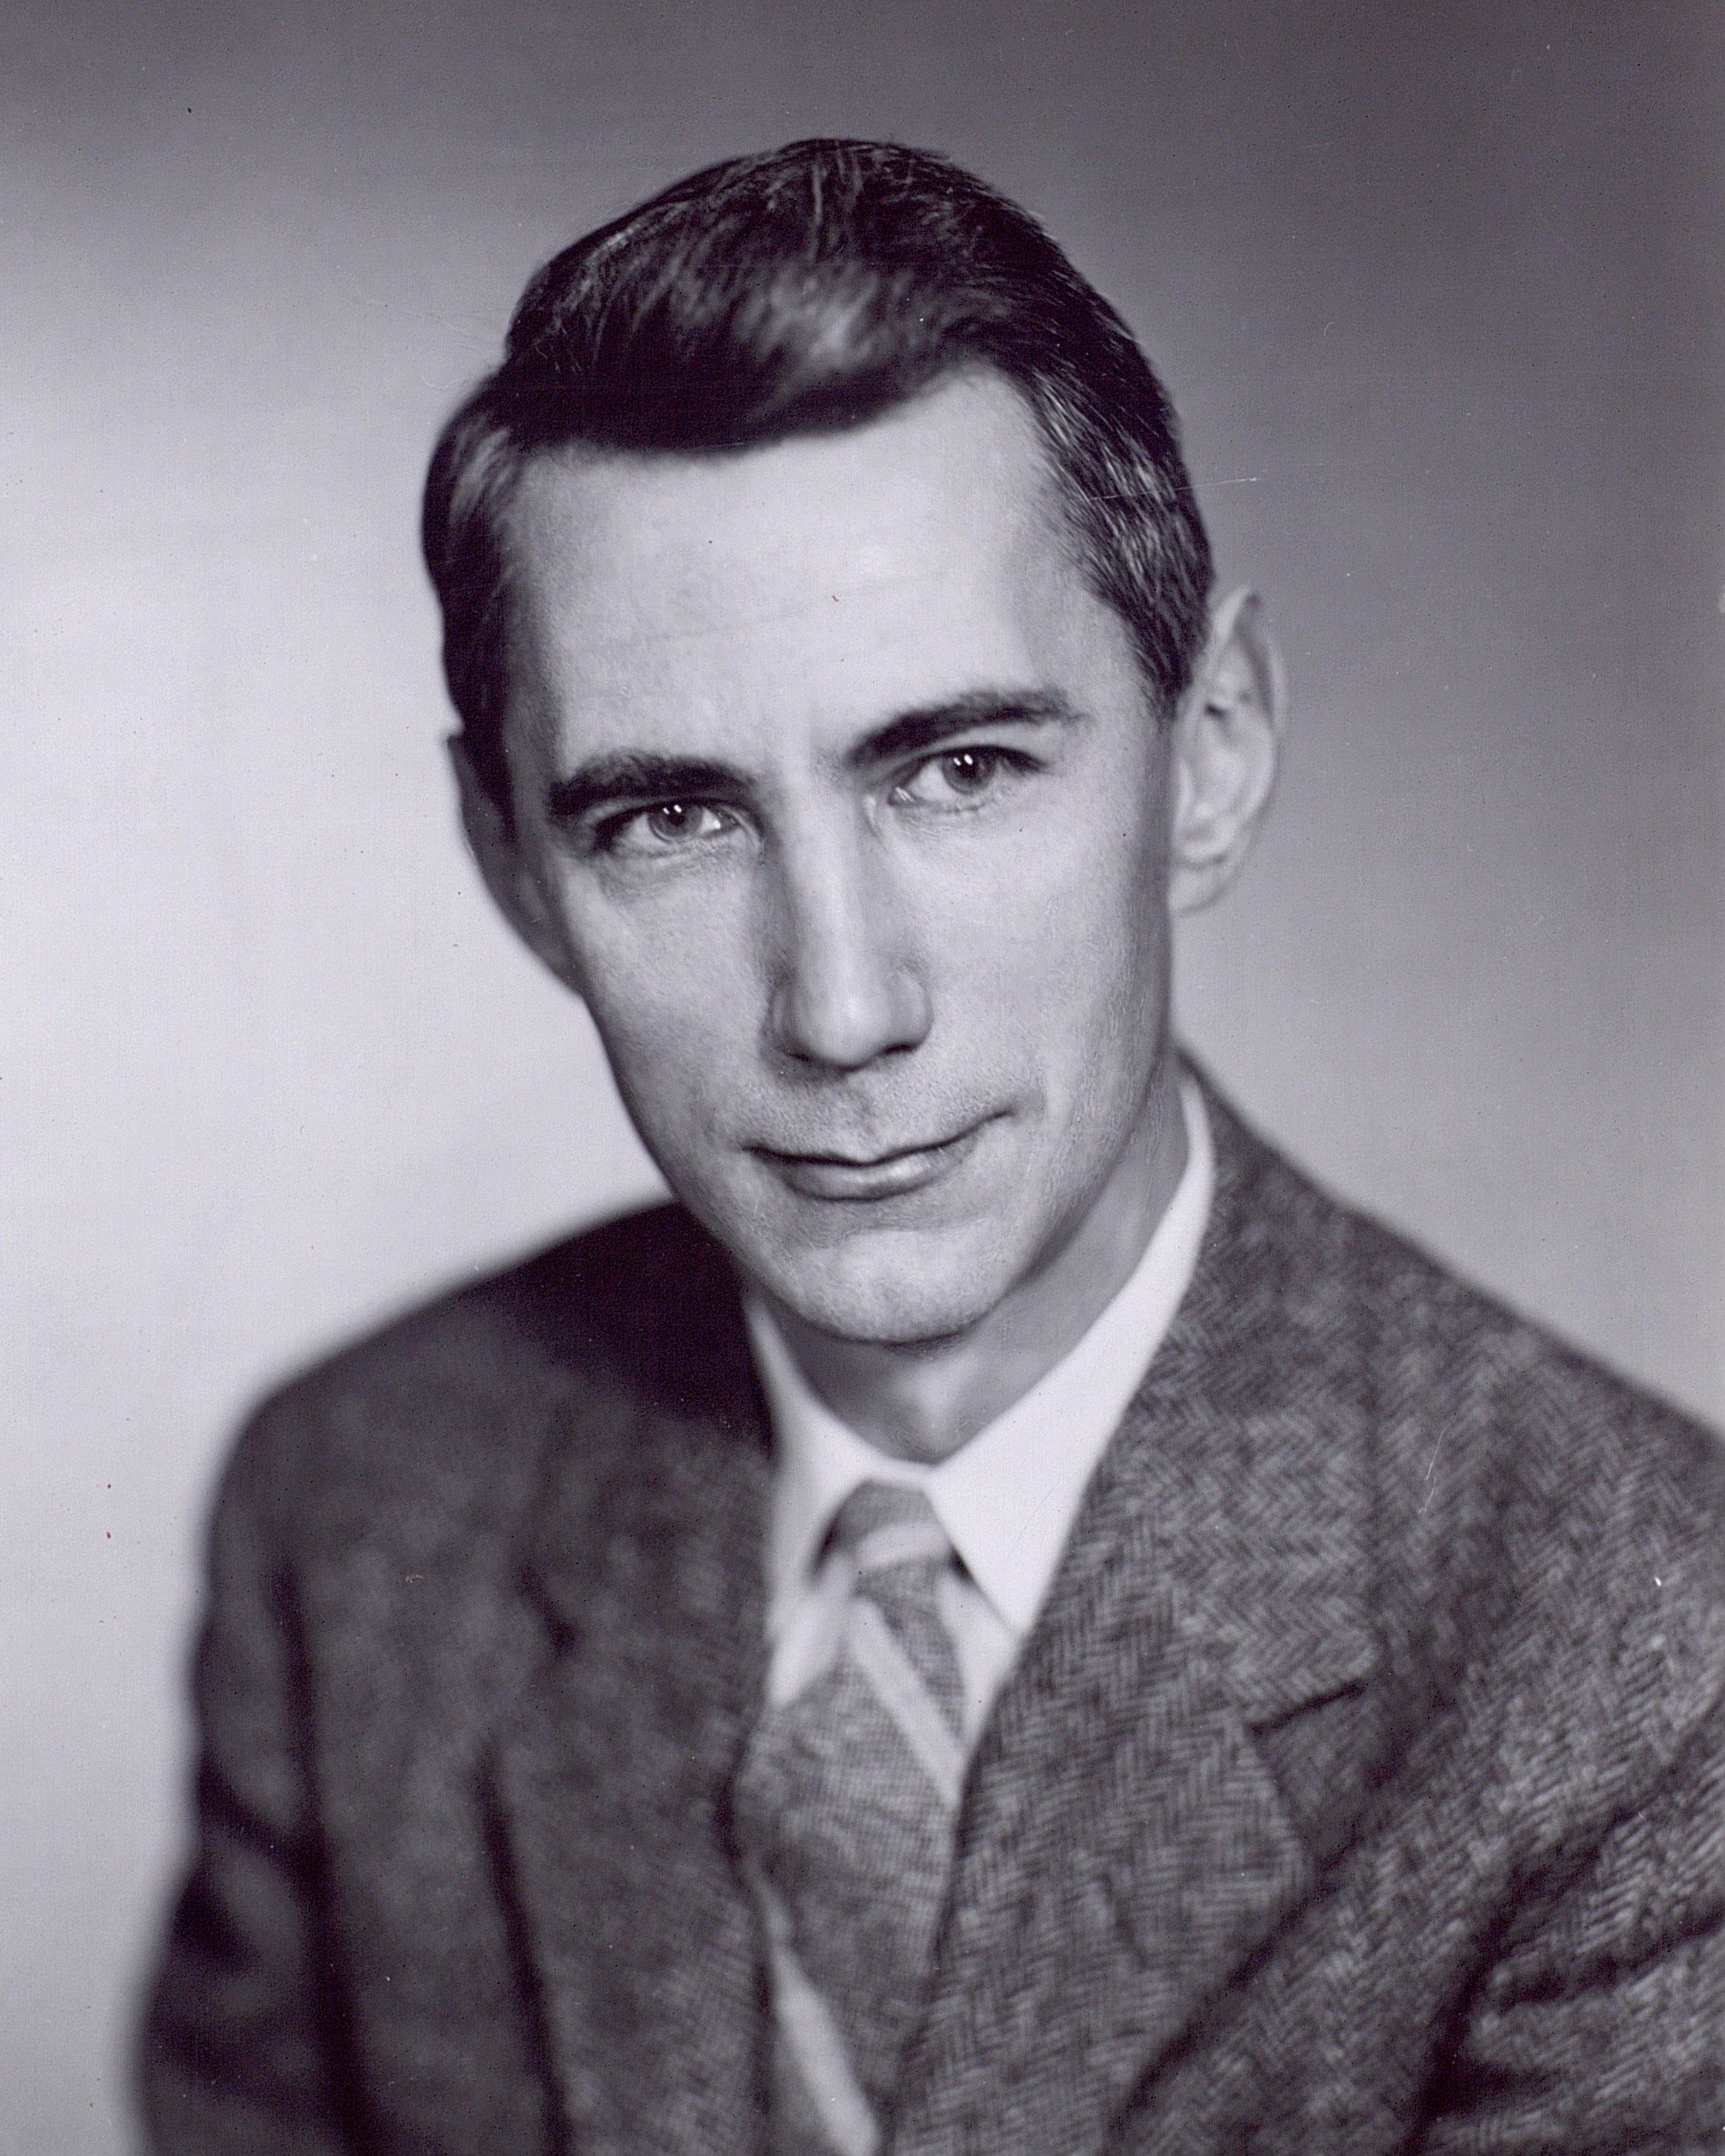
\includegraphics[width=0.25\linewidth]{images/Shannon.jpg}
    \caption{\scriptsize C.E.~Shannon. Source: By Unknown author - Tekniska Museet, CC BY 2.0, \url{https://commons.wikimedia.org/w/index.php?curid=144716444}}
    \label{Claude Shannon}
\end{figure}






\begin{theorem}[Shannon lower bound]
    For every $n>1$ there exists a function $f:\{0,1\}^n \rightarrow\{0,1\}$ that cannot be computed by a circuit of size  $\le \nicefrac{2^n}{10 n}$.
\end{theorem}


To prove this theorem, we are going to use a \emph{counting argument}. 
\begin{svgraybox}
\textbf{Counting argument}. The counting argument at its core is a use of the \emph{pigeonhole principle}, which states that we cannot place $n$ pigeons in $n-1$ pigeonholes, given that each hole can fit at most a single pigeon. Or dually, that we cannot cover $n$ holes with $n-1$ pigeons. 
\end{svgraybox}

\begin{proof}
We are going to count the number of distinct possible circuits of size at most $\nicefrac{2^n}{10 n}$, and conclude that this number is smaller than the number of possible distinct Boolean functions $f:\bits^n\to\bits$. Hence, we cannot cover all possible Boolean functions with $n$ variables with the set of circuits of size at most $\nicefrac{2^n}{10 n}$. Namely, there is a Boolean function that cannot be computed by any circuit of size at most $\nicefrac{2^n}{10 n}$.

 

\renewenvironment{claim}{%
    \vspace{6pt} 
    \noindent\textit{Claim:} % Code at the beginning
    \itshape % Italicize the text inside the environment
}{%
    \par % Code at the end (e.g., end with a paragraph break)
}

\newenvironment{proofclaim}{%
    \vspace{6pt} 
    \noindent\textit{Proof:} % Code at the beginning
}{%
    \hfill$\Box_{\rm claim}$\par\vspace{10pt} % Code at the end (e.g., end with a paragraph break)
}



\begin{claim}
We can encode a boolean circuit of size $S$ with at most $5\cdot S \log S$ bits.
\end{claim}

\begin{proofclaim}
Using adjacency list to encode a circuit of size at most $S$.   Note that since $S$ is the upper bound of the size of the circuit, we can label the gates of the circuit by numbers from $\{0,1,2,\dots,S-1\}$. Thus, every gate $i$ can be encoded by $\lceil \log S \rceil$ bits.  Each entry $i$ in the list contains at most two numbers $j,k<i\le S-1$ designating that the gates $j,k$ have both an incoming edge into the gate $i$ (if the gate $i$ is ``$\neg$'' it has fan-in one, and we need only one number). This amounts to $\le 2\cd \lceil\log S\rceil$ bits. We also need to encode the gate type ($\lor,\land,\neg$) and for this we need only two extra bits. So all in all, each cell in the list uses only $2+2\cd\lceil\log S\rceil$ many bits.
\begin{figure}[H]
    \centering
    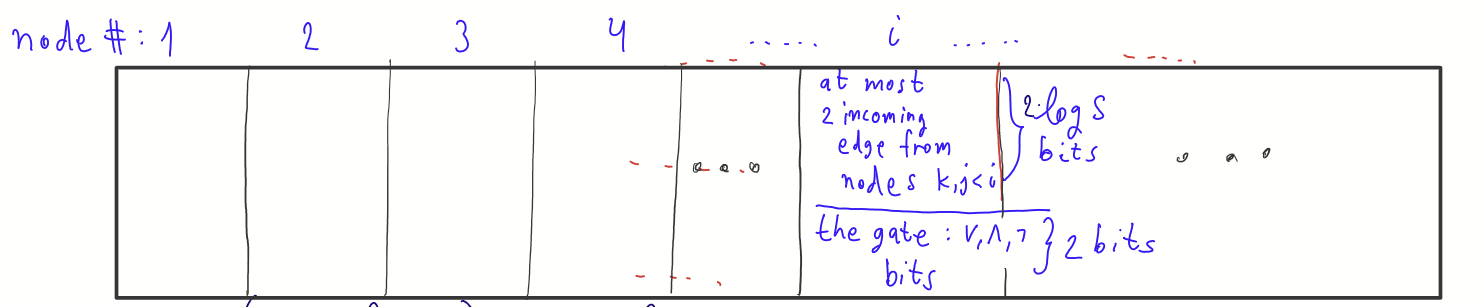
\includegraphics[width=1.1\linewidth]{images/shannon_table.png}
    \caption{The encoding scheme for a Boolean circuit of size $S$.}
    \label{fig:enter-label}
\end{figure}


We have:
$$
S \cdot(2+2 \lceil \log S \rceil) = 
2S +2S \lceil \log S \rceil \leq  4 S \ceil {\log S}\le 5S\log S.$$
\end{proofclaim}

We now show that the number of circuits of size $\leq 2^n / 10 n$ is smaller than the number of possible Boolean functions with $n$ inputs.
Thus,  there exists a Boolean function that cannot be computed by a circuit of size $\leq 2^n / 10 n$.

The number of circuits of size $S$ is bounded from above by the number of distinct codes of circuits of size $S$, which is
$$
\begin{aligned}
& \leq 2^{5 \cdot S \log S} \\
& =2^{\left(5 \cdot \frac{2^{n}}{10n} \cdot \log \left(\frac{2^n}{10n}\right)\right)}=
2^{\left(5 \cdot \frac{2^n}{10 n} \cdot(n-\log 10 n)\right)} \\
& \leq 2^{\frac{5 n}{10 n} \cdot 2^n}=2^{2^{n-1}} . 
\end{aligned}
$$
% $$
% \begin{aligned}
% & \leq 2^{9 \cdot S \log S} \\
% & =2^{\left(9 \cdot 2^{n / 10 n} \cdot \log \left(2^n / 10 n\right)\right)}=2^{\left(9 \cdot 2^n / 10 n \cdot(n-\log 10 n)\right)} \\
% & \leq 2^{\frac{9 n}{10 n} \cdot 2^n}=2^{\frac{9}{10} \cdot 2^n} . 
% \end{aligned}
% $$
But this is 
less than $2^{2^n}$ the number of distinct Boolean functions $f:\{0,1\}^n\to\{0,1\}$. 
\end{proof}

\noindent \textbf{Note}:  The reason our size lower bound is $2^n/10n$, instead for example a stronger lower bound of $2^n/c$, for some constant $c$, is that encoding a circuit is \emph{super linear} (i.e., $\Omega (n\cd\log n)$). 
Note indeed that using smaller codes for circuits amounts to stronger (i.e., bigger) lower bounds:  if we denote by $code(S)$ the maximal length needed to encode circuits of size $S$, then $2^{code(S)}$ is the number of different codes, which bounds the number of different functions computed by size $S$ circuits. In the proof we need to show that $2^{code(S)}<2^{2^n}$. Thus, as $code(S)$ gets smaller as a function of $S$, namely the encoding of circuits is more efficient, we get a better lower bound: we get that the inequality $2^{code(S)}<2^{2^n}$ holds for \emph{bigger} $S$.  


 



\subsection{Answers}








\begin{trailer}{Answer to Question \ref{quest:1}}\label{trailer:xor-circuit}
     PARITY on 4 input bits. It outputs 1 iff the number of 1's in the input is odd. I.e., it computes the XOR of $x_1, \ldots, x_4$. In other words, it computes the function $x_1+x_2+x_3+x_4 \mod 2$, where $x_i\in\bits$, for $i\in[4]$. (Understand why that is. Hint: recall that ${\neg A}\lor B$ is logically equivalent to $A\to B$. So $\neg (A\to B) \land \neg(B\to A)$ computes the XOR of $A, B$. Now, notice that this structure repeats throughout the circuit.)
\end{trailer}
%\eject



